% -----------------------------------------------
% Template for ISMIR Papers
% 2017 version, based on previous ISMIR templates

% Requirements :
% * 6+n page length maximum
% * 4MB maximum file size
% * Copyright note must appear in the bottom left corner of first page
% * Clearer statement about citing own work in anonymized submission
% (see conference website for additional details)
% -----------------------------------------------

% Anonymity: authors, GitHub links, acknowledgments

\documentclass{article}
\usepackage{ismir,amsmath,cite,url}
\usepackage{graphicx} \graphicspath{{figs/}}

\usepackage[T1]{fontenc} \usepackage[utf8]{inputenc}
\usepackage[bookmarks=false,colorlinks=true,allcolors=blue]{hyperref}
\usepackage{booktabs, threeparttable, tabularx}
\usepackage{enumitem} \setlist{itemsep=0pt,topsep=0pt,parsep=0pt,partopsep=0pt}

\usepackage{color}
\newcommand{\todo}[1]{{\color{red} #1 }}

\title{FMA: A Dataset For Music Analysis}

\oneauthor
{Kirell Benzi, \hspace{.2cm} Michaël Defferrard, \hspace{.2cm} Pierre Vandergheynst, \hspace{.2cm} Xavier Bresson}
 {{\tt michael.defferrard@epfl.ch, kirell.benzi@epfl.ch} \\
  {\tt pierre.vandergheynst@epfl.ch, xavier.bresson@epfl.ch} \\
  LTS2, EPFL, Lausanne, Switzerland}

%\threeauthors
%  {First Author} {Affiliation1 \\ {\tt author1@ismir.edu}}
%  {Second Author} {\bf Retain these fake authors in\\\bf submission to preserve the formatting}
%  {Third Author} {Affiliation3 \\ {\tt author3@ismir.edu}}

%% To make customize author list in Creative Common license, uncomment and customize the next line
\def\authorname{Kirell Benzi, Michaël Defferrard, Pierre Vandergheynst, Xavier Bresson}

\sloppy % please retain sloppy command for improved formatting
\begin{document}
\maketitle

% about 150-200 words.
\begin{abstract}
We present a new music dataset that can be used for several music analysis tasks. Our major goal is to go beyond the existing limitations of available music datasets, which are either the small size of datasets with raw audio tracks, the availability and legality of the music data, or the lack of meta-data for artists analysis or song ratings for recommender systems. Existing datasets such as GTZAN, TagATune, and Million Song suffer from the previous limitations. It is however essential to establish such benchmark datasets to advance the field of music analysis, like the ImageNet dataset which made possible the large success of deep learning techniques in computer vision. In this paper, we introduce the Free Music Archive (FMA) which contains 77,643 songs and 68 genres spanning 26.9 days of song listening and meta-data including artist name, song title, music genre, and track counts. For research purposes, we define two additional datasets from the original one: a small genre-balanced dataset of 4,000 song data and 10 genres compassing 33.3 hours of raw audio and a medium genre-unbalanced dataset of 14,511 data and 20 genres offering 5.1 days of track listening, both datasets come with meta-data and Echonest audio features. For all datasets, we provide a train-test splitting for future algorithms' comparisons.
\end{abstract}

The released dataset is composed of 100,000 tracks, xx artists, xx albums, xx hours of audio (xx GiB), 164 genres, all under permissive Creative Commons licenses.

The dataset comes with a collection of meta-data such as the song titles, artists and albums, together with full-length audio and a set of pre-computed features as well as a train/test split.

Content-based music information retrieval tasks are typically solved with a two-stage approach: engineered features are extracted from music audio signals, and are then used as input to a regressor or classifier.
Although that approach was dominant in the past, feature learning and end-to-end learning (from signal to label) have started to receive more attention from the MIR community in recent years. 
The primary goal of this dataset is to enable researchers to train large models, which require lots of training data, which could potentially avert the semantic gap currently observed between the extracted low-level features such as MFCCs and the high-level targets such as genre.
Hopefully, the release of such amount of easily accessible data will foster research which will ultimately surpass the performance ceiling observed in e.g. genre recognition, as it as been the case in computer vision with the release of ImageNet.

This paper describes the dataset and how it was created, proposes some tasks and evaluate some baselines for music genre recognition (MGR).
All the code to reproduce it as well as links to download the data and usage examples are available at \url{https://github.com/mdeff/fma}.


%%%%%%%%%%%%%%%%%%%%%%%%%%%%%%%%%%%%%%%%%%%%%%%%%%%%%%%%%%%%%%%%%%%%%%%%%%%%%%%%
\section{Introduction} % and Motivation}
%%%%%%%%%%%%%%%%%%%%%%%%%%%%%%%%%%%%%%%%%%%%%%%%%%%%%%%%%%%%%%%%%%%%%%%%%%%%%%%%


\noindent
{\bf Music Analysis Field.} Developing new mathematical models and algorithms to solve challenging real-world problems is obviously of first importance in any field of research. But such novel techniques must be evaluated and compared to the existing state-of-the-art techniques to be adopted as new standards by research communities. Evaluation and comparison require benchmark datasets to achieve their purpose, which are sometimes challenging to collect and share. In computer vision, the community has developed over the years well-established benchmark datasets such as \href{http://yann.lecun.com/exdb/mnist/}{MNIST} \cite{mnist}, \href{https://www.cs.toronto.edu/~kriz/cifar.html}{CIFAR} \cite{cifar}, or \href{http://www.image-net.org}{ImageNet} \cite{imagenet}. All these image datasets are free, legal and easily available on Internet. Such datasets have proved essential to advance the field of computer vision. The most celebrated example is the ImageNet dataset and challenge in 2012. This unprecedented dataset of 1.5M image data allowed to demonstrate the power of deep learning techniques, which was able to win the competition by a large margin over the second best. In music analysis, such benchmark datasets are not easily available and they also lack of essential information. For examples, developing deep learning techniques for music applications require the use of raw audio data, and designing recommender systems need meta-data like artist features and song ratings. Besides, the most influential competition in the field of music analysis organized every year is the Music Information Retrieval Evaluation eXchange (MIREX).\href{http://www.music-ir.org/mirex/wiki/}{MIREX} proposes several important music analysis challenges such as song identification, tag classification, music similarity and retrieval, etc. However, participants do not have access to neither the test set, nor the important train set. They must upload their code to a website that will be evaluated by the organizers. In other words, participants cannot train their analysis models on any part of the dataset. These existing shortcomings make essential the development of new music datasets to advance the field of music analysis.   \\

In contrast with other modalities such as images or text for which a wealth of content is available, the lack of a large-scale and easily available dataset for MIR has hindered research on data-heavy models such as Deep Learning (DL).

\noindent
{\bf Available music datasets and their limitations.} In music analysis, three datasets have been widely used by the international society for music information retrieval (\href{http://www.ismir.net/}{ISMIR}): the GTZAN, TagATune, and MSD (Million Song Dataset) datasets. However each dataset come with some limitations:
We discuss below some of the most related datasets, see \tabref{tab:datasets} for a more comprehensive list.
\tabref{tab:datasets} shows the most common datasets used for audio-based / content-based MIR.
\begin{description}
	\item[GTZAN] \cite{gtzan} is a collection of 1000 songs with 10 music genres. Each song is represented by a 22,050Hz Mono 16-bit wav audio file of 30sec. It is the first benchmark MGR dataset to have been made publicly available, and as a result continues to be the most used public dataset for MGR \cite{mgr_eval}. A complete study, and critic, of this dataset was done in \cite{gtzan_critic_1}, and the dataset is available online. The main limitations of GTZAN is the legality of the dataset, the small size, no complete meta-data regarding artist names and song titles, and no additional meta-data like ratings.
	\item[MagnaTagATune] \cite{magnatagatune} is a popular dataset of 5,405 source songs from 230 artists, cut in 25,863 clips. The music was collected from the \href{https://magnatune.com/}{Magnatune} label and was tagged using the \href{http://tagatune.org/}{TagATune} game. The dataset includes meta-data, audio features and raw audio, although the 16 kHz, 32kbps, mono mp3 are of poor audio quality.
	\item[The Million Song Dataset (MSD)] \cite{msd} is a free and legal collection of 1 million music songs. Each song data is composed of high-level and medium-level audio features provided by  Echonest service and meta-data like artist name, song title, track genre, etc. It has its own dedicated website with related code and additional datasets. The very large scale of this music dataset would make it an ideal candidate for deep learning, which works best with large datasets. However, deep learning techniques work directly on the raw data (audio tracks in this case, like raw image pixels in computer vision) and not on pre-processed audio features given by Echonest. This prevents the application of deep learning on this dataset. Finally, Echonest reassigned the indexing of the MDS songs with its database, which henceworth makes (almost) impossible the use of the most music recent features developed by Echonest.
		While researchers have been able to download sample audio from the online service \href{https://www.7digital.com}{7digital.com} and extract features by themselves, the process is tedious \cite{msd_features}.
	\item[AudioSet] \cite{audioset} is a dataset of 2.1 million annotated 10-second sound clips associated with 527 classes. The ontology is quite broad and covers sounds from music to cars, engines or animals. The raw audio is however not included and has to be downloaded from Youtube. It is not clear of what happens if a referenced video gets deleted.
\end{description}

\begin{table}
	\centering
	\begin{threeparttable}
	\begin{tabular}{lrrcc}
		\toprule
		dataset & \#clips & \#artists & year & audio \\
		\midrule
		\href{https://staff.aist.go.jp/m.goto/RWC-MDB/}{RWC} \cite{RWC} & 465 & - & 2001 & yes \\
		\href{http://calab1.ucsd.edu/~datasets/cal500/}{CAL500} \cite{cal500} & 500 & 500 & 2007 & yes \\
		\href{http://mtg.upf.edu/ismir2004/contest/tempoContest/node5.html}{Ballroom} \cite{ballroom} & 698 & - & 2004 & yes \\
		\href{http://ismir2004.ismir.net/genre_contest/}{ISMIR2004} & 729 & - & 2004 & yes \\
		\href{https://marsyasweb.appspot.com/download/data_sets/}{GZTAN} \cite{gtzan} & 1,000 & $\sim300$ & 2002 & yes \\
		\href{http://www.cp.jku.at/datasets/musiclef/}{MusiClef} \cite{musiclef} & 1,355 & 218 & 2012 & yes \\
		\href{https://labrosa.ee.columbia.edu/projects/artistid/}{Artist20} \cite{artist20} & 1,413 & 20 & 2007 & yes \\
		\href{http://www-ai.cs.uni-dortmund.de/audio.html}{Homburg} \cite{garageband} & 1,886 & - & 2005 & yes \\  % GarageBand
		\href{http://www.seyerlehner.info/index.php?p=1_3_Download}{Unique} & 3,115 & - & 2010 & no \\
		\href{http://www.seyerlehner.info/index.php?p=1_3_Download}{1517-Artists} & 3,180 & 1,517 & 2010 & yes \\
		\href{http://www.ppgia.pucpr.br/~silla/lmd/}{LMD} \cite{lmd} & 3,227 & - & 2007 & no \\
		\href{http://anasynth.ircam.fr/home/media/ExtendedBallroom}{EBallroom} \cite{extballroom} & 4,180 & - & 2016 & no\tnote{1} \\
		\href{https://labrosa.ee.columbia.edu/projects/musicsim/uspop2002.html}{USPOP} \cite{uspop} & 8,752 & 400 & 2003 & no \\
		\href{http://calab1.ucsd.edu/~datasets/cal10k/}{CAL10k} \cite{cal10k} & 10,271 & 4,597 & 2010 & no \\ % Swat10k
		\href{http://mirg.city.ac.uk/codeapps/the-magnatagatune-dataset}{TagATune} \cite{magnatagatune} & 25,863\tnote{2} & 230 & 2009 & yes\tnote{3} \\ % MagnaTagATune
		\href{http://jmir.sourceforge.net/index_Codaich.html}{Codaich} \cite{codaich} & 26,420 & 1,941 & 2006 & no \\ % paper 20,849
		\bf \href{https://github.com/mdeff/fma/}{FMA} & \bf 110,000 & \bf - & \bf 2017 & \bf yes \\
		\href{http://www.omras2.org/}{OMRAS2} \cite{omras} & 152,410 & 6,938 & 2009 & no \\
		\href{https://labrosa.ee.columbia.edu/millionsong/}{MSD} \cite{msd} & 1,000,000 & 44,745 & 2011 & no\tnote{1} \\
		\href{https://research.google.com/audioset/}{AudioSet} \cite{audioset} & 2,100,000 & - & 2017 & no\tnote{1} \\
		\bottomrule
	\end{tabular}
	\begin{tablenotes}
		\item[1] Audio can be downloaded from a web service. % \url{www.ballroomdancers.com} \url{7digital.com} \url{youtube.com}
		\item[2] The 25,863 clips come from 5,405 songs.
		\item[3] Low quality 16 kHz, 32kbps, mono mp3.
	\end{tablenotes}
	\end{threeparttable}
	\caption{Comparison with some other datasets.}
	\label{tab:datasets}
\end{table}

% Lists of datasets:
% * http://www.audiocontentanalysis.org/data-sets/
% * A Survey of Evaluation in Music Genre Recognition

% TODO licensing

\begin{table*}[t]
	\centering
	\begin{threeparttable}
		\begin{tabular}{lr
			>{$}r<{$}
			@{}>{${}={}$}c@{}
			>{$}l<{$}
			>{$}c<{$}
			cc}
		\toprule
		Dataset & \#samples & \multicolumn{3}{c}{Dimensionality} & \multicolumn{3}{c}{Size} \\
		\cmidrule{6-8}
				&           & \multicolumn{3}{c}{}               & \text{scale} & [GB] & [days] \\
		\midrule
		\href{http://mirg.city.ac.uk/codeapps/the-magnatagatune-dataset}{TagATune} \cite{magnatagatune} &
			25,863 & 29\cdot16\cdot10^3\cdot1 && 4.6\cdot10^5 & 1.2\cdot10^{10} & 3 & 8.7 \\ % MagnaTagATune
		\href{https://research.google.com/audioset/}{AudioSet} \cite{audioset} \tnote{1} &
			2,100,000 & 10\cdot44\cdot10^3\cdot2 && 8.8\cdot10^5 & 1.8\cdot10^{12} & - & 243 \\
		\href{https://labrosa.ee.columbia.edu/millionsong/}{MSD} \cite{msd} \tnote{2} &
			1,000,000 & 49\cdot27\cdot10^3\cdot2 && 2.6\cdot10^6 & 2.6\cdot10^{12} & 625 & 541 \\
		\href{https://github.com/mdeff/fma/}{FMA} \tnote{3} &
			110,000 & 180\cdot44\cdot10^3\cdot2 && 1.6\cdot10^7 & 1.7\cdot10^{12} & 900 & 229 \\
		\midrule
		\href{http://yann.lecun.com/exdb/mnist/}{MNIST} \cite{mnist} &
			70,000 & 28\cdot28\cdot1 && 7.8\cdot10^2 & 5.5\cdot10^{7\phantom0} & 0.011 & - \\
		\href{https://www.cs.toronto.edu/~kriz/cifar.html}{CIFAR-10} \cite{cifar} &
			60,000 & 32\cdot32\cdot3 && 3.0\cdot10^3 & 1.8\cdot10^{8\phantom0} & 0.16 & - \\
		\href{http://www.image-net.org}{ImageNet} \cite{imagenet} \tnote{4} &
			14,000,000 & 482\cdot415\cdot3 && 6.0\cdot10^5 & 8.4\cdot10^{12} & 1000 & - \\
		\bottomrule
	\end{tabular}
	\begin{tablenotes}
		\item[1] \href{https://support.google.com/youtube/answer/6039860}{YouTube recommended} sample rate for music videos.
		\item[2] Average duration and sample rate. Most excerpts from \href{https://www.7digital.com}{7digital} are 30 or 60s and 22 or 44kHz \cite{msd_features}.
		\item[3] Average duration and sample rate. See \todo{ad} for details.
		\item[4] Average resolution. Although most applications resize or crop to $256\cdot256$.
	\end{tablenotes}
	\end{threeparttable}
	\caption{Size comparison. Dimensionality is (length $\cdot$ sample rate $\cdot$ \#channels) for audio and (xdim $\cdot$ ydim $\cdot$ \#channels) for images. Scale is the number of samples times the dimensionality. Size is for a (zipped) archive of all mp3 or jpeg in GB, which is an indication of the quantity of information, e.g. duration or quality. The last column is the number of days to listen to the whole available audio.}
	\label{tab:size}
\end{table*}

% table quality

Our differentiating factors:
\begin{description}
	\item[Large scale.] Large datasets are needed to avoid overtraining and to effectively learn models that incorporate the ambiguities and inconsistencies that one finds with genre. While FMA is not the largest in term of number of clips, every other dataset with readily available quality audio are two orders of magnitude smaller. A possibly more important size metric here is the total amount of audio, i.e. the sum of the lengths of all clips, in which FMA is in a much better position (see \tabref{tab:size}). For comparison, ImageNet \cite{imagenet}, the largest benchmark dataset in computer vision features 14 million images. Despite a much larger collection, the amount of data is comparable to that of MSD or FMA because of the smaller dimensionality, as shown in \tabref{tab:size}. For statistical learning algorithms, the scale of FMA and MSD is thus comparable to ImageNet.
	\item[Permissive licensing.] MIR research has historically suffered from the lack of publicly available benchmark datasets. Most of these issues stem from the commercial interest in music by record labels, and therefore imposed rigid copyright. All songs are licensed under Creative Commons by the artists and can thus be redistributed. The meta-data produced by ourselves are released under \todo{Creative Commons ?? v4} and the code under an MIT license.
* In contrast with images or text for which plenty of data is available online
	\item[Audio.] most of the largest datasets are distributed with features, sometimes computed by commercial services like the Echonest. Researchers are wary of those proprietary features and have seek to compute features themselves, e.g. on the MSD \cite{msd_features}. In contrast, FMA provides audio for each song.
	\item[High quality audio.] full-length original audio uploaded by the artist. Stereo mp3 with bitrates varying between x. Audio, if released or available to download, is usually clips of 10 to 30 seconds. To our knowledge, none of the released datasets up to this date come with full-length audio.
	\item[Future proof]: all audio and meta-data can be downloaded as ZIP archives, no need to scrap the web yourself. They are checksummed, have a DOI and are hosted on \href{https://zenodo.org}{zenodo.org}, a long-term digital archive powered by CERN. We thus alleviate the risks of tracks to become unavailable, to change without notice or for online services to shut down.
	% Western / commercial music, how to qualify broadness?
	\item[Reproducible]: we share all the code used to (i) collect the dataset, (ii) analyze it, (iii) extract the sub-sets, (iv) compute the features and (v) the baselines, so that it can be reproduced or extended. As the original data and APIs are public, anybody can recreate the dataset.
	\item[Easy to work with]: working with the dataset only requires to download some archives. Moreover, we provide an helper \href{https://pypi.python.org/pypi/freemusicarchive}{Python package} and some usage examples in the \texttt{usage.ipynb} Jupyter notebook to quick start using the data.
\end{description}

% Magnatagature dead links: http://tagatune.org/Datasets.html http://tagatune.org/Magnatagatune.html
% Announcement: https://musicmachinery.com/2009/04/01/magnatagatune-a-new-research-data-set-for-mir/

% TODO: talk about related datasets
% * SecondHandSongs dataset -> cover songs
% * musiXmatch dataset -> lyrics
% * Last.fm dataset -> song-level tags and similarity
% * Taste Profile subset -> user data
% * thisismyjam-to-MSD mapping -> more user data
% * tagtraum genre annotations -> genre labels
% * Top MAGD dataset -> more genre labels

The sets in \tabref{tab:datasets} are either smaller, either provide audio through online services.

From \tabref{tab:datasets}, it is obvious that the main problem is that larger datasets do not come with the audio. Either they contain only features derived from the audio, either they provide links for the user to download the audio from an online service. The problem with the former is that researchers are stuck with the set of chosen features, while the later make no assurance that the files or services are not gonna disappear or change without notice.
We see from \tabref{tab:datasets} that most of the smallest datasets come with audio while most of the largest don't. That state of affair is due to copyright laws which forbid the redistribution of audio. The solution to that problem is to aim for tracks released under permissive licenses, such as \href{https://creativecommons.org/}{Creative Commons}.

Creative Commons: MagnaTagATune
Proprietary, non-redistributable: MSD, AudioSet?

% Do not present like this because we might want representativeness. Which would necessarily include commercial music.

%{\bf What would be the requirements for an ideal music dataset?} \\
%(1) Availability of raw audio tracks like 30sec or more,\\
%(2) Availability of meta-data such as genres, artist, title, year, lyrics, users' ratings, users' comments, etc,\\
%(3) Large-scale dataset to be able to sample the high-dimensional distribution of music genres\\
%(4) Free and easy access of the dataset,\\
%(5) Legality of the dataset, no copyright issue with e.g. open access licence.\\


%%%%%%%%%%%%%%%%%%%%%%%%%%%%%%%%%%%%%%%%%%%%%%%%%%%%%%%%%%%%%%%%%%%%%%%%%%%%%%%%
\section{The Dataset} %Introducing the FMA dataset}
%%%%%%%%%%%%%%%%%%%%%%%%%%%%%%%%%%%%%%%%%%%%%%%%%%%%%%%%%%%%%%%%%%%%%%%%%%%%%%%%


% Describe what it is, what are the meta-data and features.

%\subsection{The Free Music Archive}

The dataset is a dump of the \href{https://freemusicarchive.org/}{Free Music Archive} (FMA), an interactive library of high-quality, legal audio downloads directed by \href{https://wfmu.org/}{WFMU}, the longest-running freeform radio station in the United States.
The archive is funded by the New York State Music Fund, the MacArthur Foundation, the National Endowment for the Arts, and from the project's users.
The website provides a large catalog of artists and high-quality mp3-encoded songs, hand-picked by established audio curators. Each song is legally free to download as artists decided to release their works under a permissive license, most tracks being released under a \href{https://creativecommons.org/}{Creative Commons license} which allows redistribution of the audio. Cheyenne Hohman, the director of the FMA, \href{http://freemusicarchive.org/member/cheyenne_h/blog/100000_SONGS}{announced} in July 2016 that the website had reached the landmark of 100,000 songs.
Inspired by Creative Commons and the open-source software movement, the FMA provides a legal and technological platform for curators, artists, and listeners to harness the potential of music sharing. While the archive is free and open to anyone, written and audio content is curated, and permission to upload or edit content is granted on an invitation basis \cite{art:MossFMA}.

\subsection{Creation} % Collection, Creation, Generation
% How it was collected.

\begin{table}
	\centering
	\begin{tabular}{|ll|}
		\hline
		track\_id & track\_title \\
		album\_title & artist\_name \\
		\hline
	\end{tabular}
	\caption{List of per-song meta-data obtained from the FMA.}
	\label{tab:metadata}
\end{table}

Song meta-data, such as the title, album, name of the artist, genres as well as some usage statistics, was crawled using the available \href{https://freemusicarchive.org/api}{API}. See \tabref{tab:metadata} for a list and \texttt{webapi.ipynb} for how to query the API with our helpers. The collected meta-information is stored in the \texttt{tracks.json} table, which \tabref{tab:tracks} shows an excerpt. Additionally, the used genre hierarchy, shown in \tabref{tab:genres}, was collected and stored in \texttt{genres.json}. Audio was then downloaded over HTTP. The collection of FMA was done in \todo{April 2016}, and the size of the dataset at this time was 89,912 songs.

\todo{Top-level genres.} Then, we created a top genre by simply picking the first genre in the original list of track genres provided by the artists.

%\subsection{Data Cleaning}

\todo{Adjust when redone.}
As a first filtering, we kept the data that has audio tracks, reducing the size to 86,886 music data. 
We removed data without genre information, giving 79,947 song data.
At this stage the number of genres is 138, but half have only a few samples. Thus we decided to only retain the genres with more than 100 samples. This defines a dataset of 77,643 music data with 68 genres. We further cleaned the dataset by removing tracks which belong to ``non-standard'' music genres like 'Noise', 'Garage', 'Sound Collage', 'Singer', 'Audio Collage', 'Glitch', 'Unclassifiable', 'Lo-Fi', 'Spoken', 'Poetry', 'Talk Radio', 'Avant-Garde', 'Experimental', 'Ambient', and 'Field Recording'. We also suppressed the songs with the title 'Untitled'. Besides, we decided to cut the long tail of the power law distribution by removing songs of genres with less than 300 songs.

The FMA\_large dataset of 77,643 data contains songs of 30sec length, and artist name, track title, track genres, track listens as meta-data. Our original motivation was to give the full audio tracks, not limited to 30sec, but the size of the whole music tracks is 806.8GB (for approximatively 256 days of music listening) making the hosting a challenging issue.

See \texttt{generation.ipynb} for full details.

\begin{table*}
	\tiny
	\centering
	\begin{tabular}{lrlrllll}
	\toprule
	 fma\_id &                                             artist &  play\_count &                                              title &                                             genres &            top\_genre  \\
	 \toprule
		10 &                                          Kurt Vile &       42936 &                                            Freeway &                                              [Pop] &                  Pop  \\
		134 &                                               AWOL &         880 &                                       Street Music &                                          [Hip-Hop] &              Hip-Hop  \\
		 142 &                    Alec K. Redfearn \& the Eyesores &         670 &                               Punjabi Watery Grave &                                             [Folk] &                 Folk  \\
		 236 &                                       Banana Clipz &        6695 &                              Push Am (Left, Right) &                              [Electronic, African] &           Electronic  \\
		 237 &                                          Barnacled &        1056 &                    Garbage and Fire &                                             [Jazz] &                 Jazz  \\
		 461 &                              Cantonement Jazz Band &        3933 &                                           Bessemer &                               [Blues, Jazz: Vocal] &                Blues  \\
		824 &                     Here Comes A Big Black Cloud!! &         391 &                                         Black Mold &          [Rock, Loud-Rock, Psych-Rock, Indie-Rock] &                 Rock  \\
		 825 &                     Here Comes A Big Black Cloud!! &        1847 &                                        Death March &          [Rock, Loud-Rock, Psych-Rock, Indie-Rock] &                 Rock  \\
		837 &                                          Heroin UK &         146 &                                           DopeSick &                                             [Rock] &                 Rock \\
		 889 &                                 Illusion of Safety &         163 &                                          Wasteland &                                       [Electronic] &           Electronic  \\
		 896 &                                        Impediments &        1542 &                                               2012 &                                  [Punk, Power-Pop] &                 Punk  \\
			  992 &                                      Jason Willett &         560 &                   Beautiful Song w/ kick drum solo &                                             [Rock] &                 Rock  \\
	\bottomrule
	\end{tabular}
	\caption{Some rows and columns of the \texttt{tracks.json} table. \todo{representative and varied}}
	\label{tab:tracks}
\end{table*}

\subsection{Content} \label{sec:content}
% Figures and tables from analysis.ipynb
% TODO audio properties: samplerate (% 44kHz), bitrate (% 128, VBR), channels (% mono, stereo)

All tracks come with the meta-data listed in \tabref{tab:metadata}, although some values may be missing.
All audio tracks are mp3-encoded with sampling rate of 44,100Hz, bit rate 128kb/s, and in stereo. 

%\subsubsection{Genres}

While it is difficult to construct a hierarchy of genres, we follow that of our source. \tabref{tab:genres} and \figref{fig:genres} show the distribution of the \todo{??} most common genres. As often encountered with natural categories, it obeys a power law.
See \texttt{analysis.ipynb} for more details.

\begin{table}
	\centering
	\begin{tabular}{cclc}
		\toprule
		ID & Parent & Genre & \#songs \\
		\midrule
		4 & None & Electronic & 50,000 \\
		4 & None & Electronic & 50,000 \\
		4 & None & Electronic & 50,000 \\
		\midrule
		45 & 2 & Psych-Rock & 500 \\
		45 & 2 & Psych-Rock & 500 \\
		45 & 2 & Psych-Rock & 500 \\
		\bottomrule
	\end{tabular}
	\caption{Number of songs per genre. Top part is the 16 top-level genres, bottom part is the second- and third-level genres.}
	\label{tab:genres}
\end{table}

\begin{figure}
	\centering
	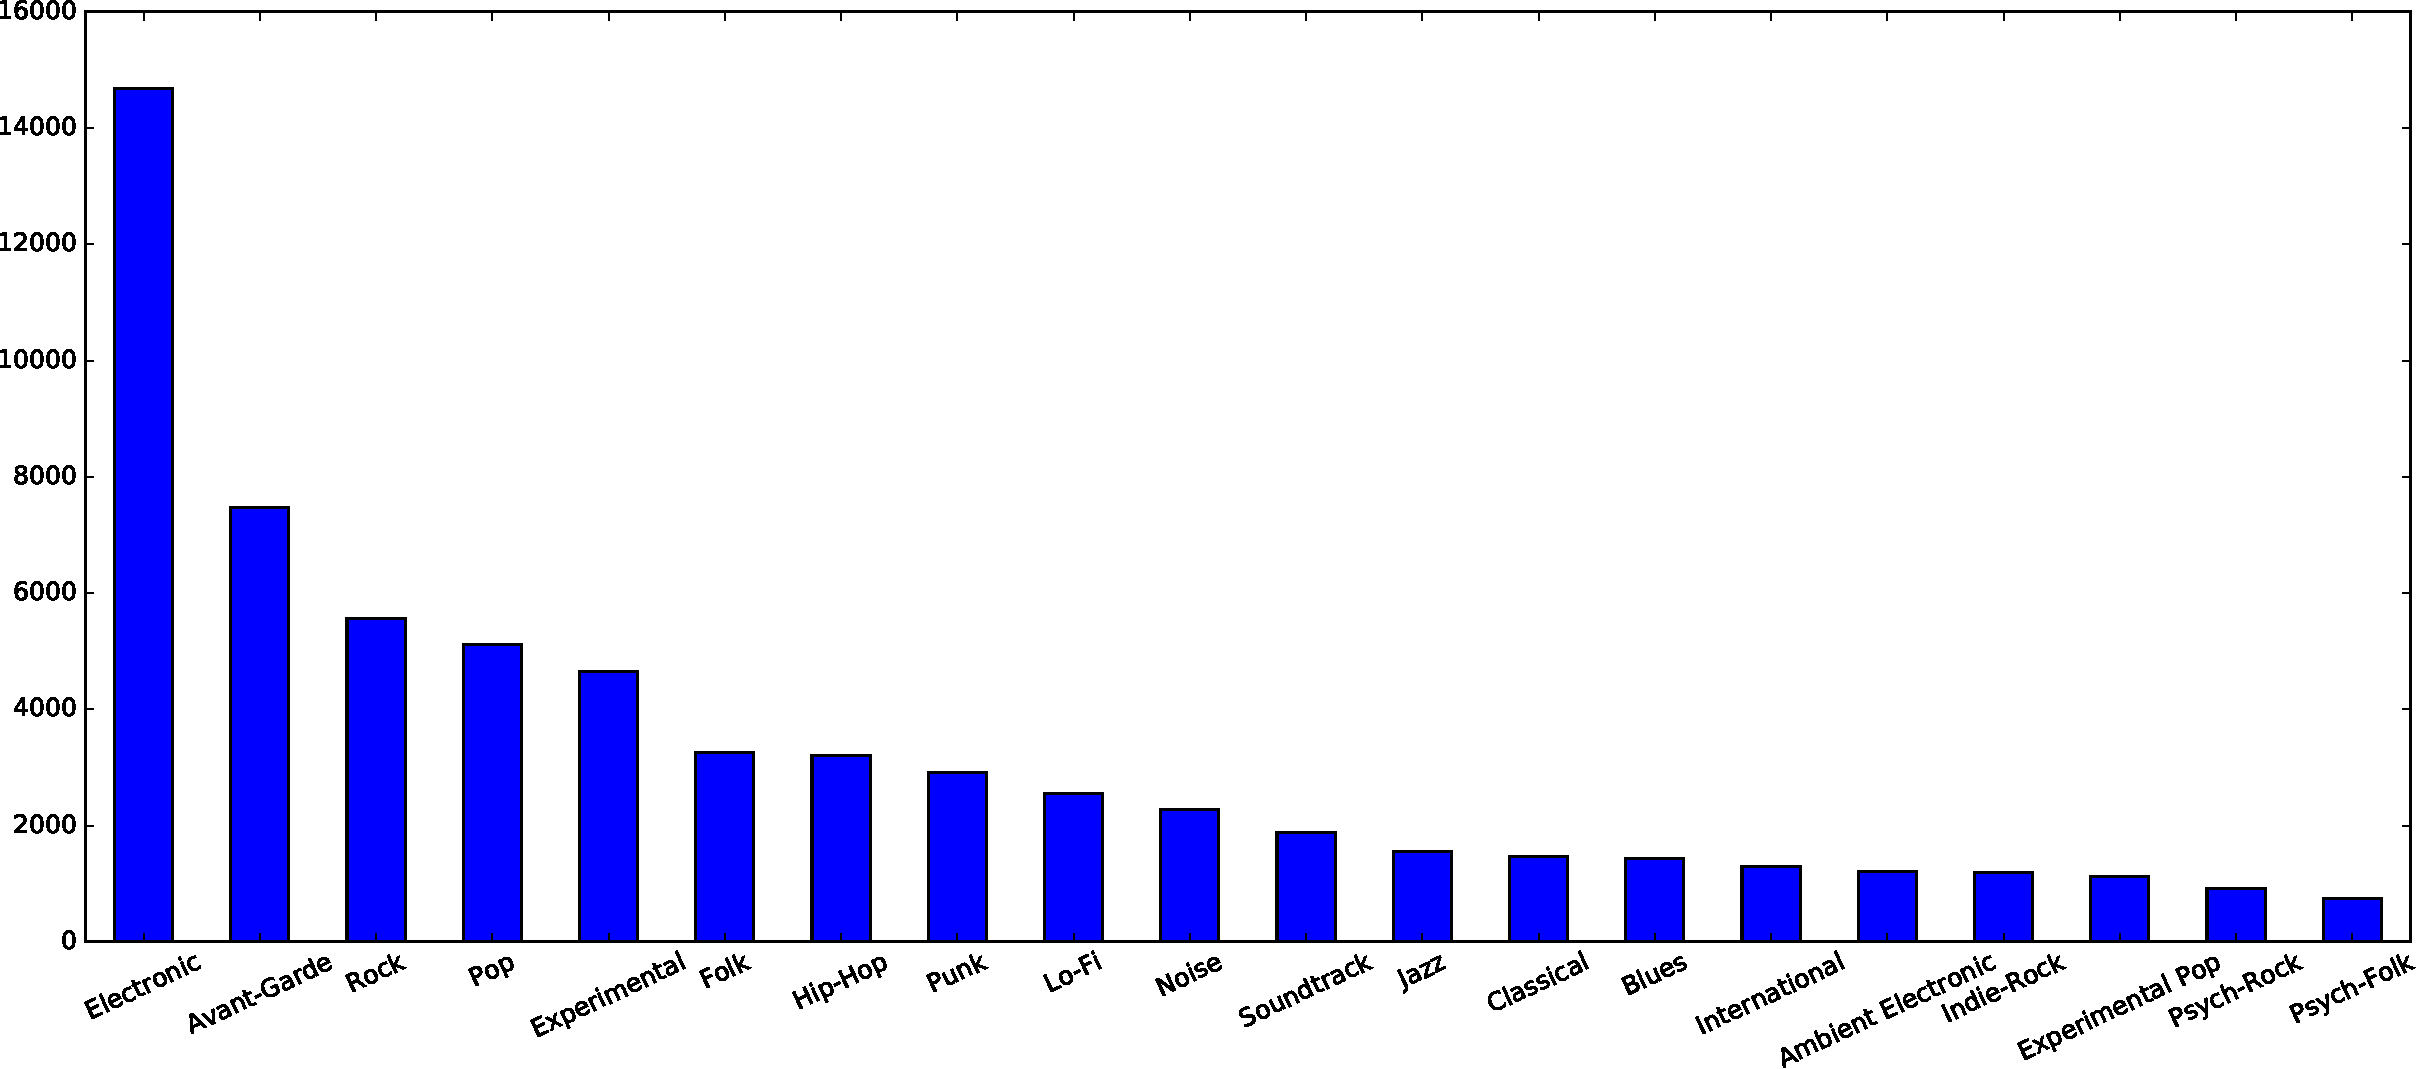
\includegraphics[width=\linewidth]{histo_large.pdf}
	\caption{Power law distribution of the top 20 genres.}
	\label{fig:genres}
\end{figure}

\subsection{Features} % Feature sets

We extracted a wide range of audio features from the audio, using the \href{https://github.com/librosa/librosa}{librosa} Python library. An overview
on these features is given in \tabref{tab:features}.
In addition, a number of descriptive medium-level and high-level audio features extracted by \href{http://the.echonest.com/}{The Echo Nest}, a music platform for developers and media companies, are provided for some tracks. These features include tempo, loudness, timings of fade-in and fade-out, and MFCC-like features for a number of segments.
Those features can be obtained either by uploading the songs to their website, which are then analyzed and sent back to the user, or simply retrieved from their database if the songs are known to them, i.e. they were analyzed before. All of which can be done through an \href{http://developer.echonest.com}{API}. In our case, we only retrieved features from songs which were already in their database.
See \texttt{features.ipynb} for more details.

\begin{table}
	\centering
	\begin{tabular}{llr}
		\toprule
		Feature set & Extractor & Dimensionality \\
		\midrule
		MFCCs \cite{mfcc} & librosa & 26 \\
		MFCCs \cite{mfcc} & librosa & 26 \\
		MFCCs \cite{mfcc} & librosa & 26 \\
		\bottomrule
	\end{tabular}
	\caption{Overview of features extracted from the FMA samples.}
	\label{tab:features}
\end{table}

\subsection{Splits}

A train / test split is proposed to make research on the FMA reproducible.
Below are the constraints we followed:
\begin{enumerate}
	\item For each genre, we randomly split train and test songs with the same ratio 80-20\%.
	\item We forced an artist to be either in the train set, or the test set (meaning the artist's songs cannot be in both train and test sets).
	\item We filled alternatively the train set and test set in the descending order of the count of artist songs. This forces the two sets to have the same distribution of songs per artist.
\end{enumerate}
A track is assigned in train or split for all the subsets and the above constraints are satisfied for all sets. See \texttt{generation.ipynb} for full details.

\subsection{Subsets} \label{sec:subsets}

\begin{table}
	\centering
	\begin{tabular}{lrrccc}
		\toprule
		dataset & clips & genres & length & \multicolumn{2}{c}{Size} \\
		\cmidrule{5-6}
		        &         &          &  [s]   & [GB] & [days] \\
		\midrule
		small  &   4,000 & 10  & 30    & 3.4  & 1.4  \\
		medium &  14,511 & 20  & 30    & 12.2 & 5.1  \\
		large  & 110,000 & 164 & 30    & 90   & 26.9 \\
		huge   & 110,000 & 164 & <1800 & 900  & 229  \\
		\bottomrule
	\end{tabular}
	\caption{Proposed subsets of the FMA.}
	\label{tab:subsets}
\end{table}

Finally, for the dataset to be useful as a development set or for people with lower computational resources, we propose the following subsets, each of which is a subset or the larger set:
\begin{enumerate}
	\item \textbf{Large}: this is the full dataset except audio is 30 seconds clips extracted from the middle of the tracks.
	\item \textbf{Medium}: all tracks which have Echonest features.
	\item \textbf{Small}: tracks from 10 top-level genres, balanced with 400 tracks per genre, 1 genre per track. This subset is similar to the very popular GTZAN in terms of size and genre distribution with the added benefits of the FMA, that is meta-data, pre-computed features and copyright-free audio.
\end{enumerate}
\tabref{tab:subsets} highlights the main differentiating factors between the proposed subsets. See \texttt{analysis.ipynb} for an analysis of the subsets' content similar to that shown in \secref{sec:content}.


%%%%%%%%%%%%%%%%%%%%%%%%%%%%%%%%%%%%%%%%%%%%%%%%%%%%%%%%%%%%%%%%%%%%%%%%%%%%%%%%
\section{Proposed usage} % tasks, usage, problems
%%%%%%%%%%%%%%%%%%%%%%%%%%%%%%%%%%%%%%%%%%%%%%%%%%%%%%%%%%%%%%%%%%%%%%%%%%%%%%%%
% List some MIR tasks and propose some who can be done with that dataset

% MSD: metadata analysis, artist recognition, automatic music tagging, recommendation, cover song recognition, lyrics, limitations


genre classification, mood classification, artist identification/recognition, instrument recognition, music annotation (tags),
Artist Identification, Genre classification, Mood Classification, Instrument identification, Music Similarity, Autotagging, Automatic playlist generation

Can be down: genre, artist, popularity prediction, tags, year prediction
% Cannot: mood, style, annotations

% TODO
% Problems
% Genre classif / mutli-genre classif
% Recommendation
% Play count prediction
% Covers: generate covers per genre / artist

Meta-data analysis: which genres are artists contributing to, drift in time, curators.
It would also be interesting to study how good does it represent mainstream music.

As it happened with e.g. the MSD, people may find and link other sources of data with the dataset, such as lyrics or tags associated to the songs, e.g. from last.fm.

We propose three genre classification problems of varying difficulty.

\begin{enumerate}
	\item Easy, based on \texttt{fma\_small.zip}: 10 top-level genres, balanced with 400 tracks per genre, 1 genre per track
	\item Medium, based on \texttt{fma\_medium.zip}: all 16 top-level genres, unbalanced with x-y tracks per genre, multiple genres per track
	\item Hard, based on \texttt{fma\_large.zip}: all 164 genres, unbalanced with x-y tracks per genre, multiple genres per track
\end{enumerate}

Training / testing division.


%%%%%%%%%%%%%%%%%%%%%%%%%%%%%%%%%%%%%%%%%%%%%%%%%%%%%%%%%%%%%%%%%%%%%%%%%%%%%%%%
\section{Genre Recognition} % MGR, Baselines
%%%%%%%%%%%%%%%%%%%%%%%%%%%%%%%%%%%%%%%%%%%%%%%%%%%%%%%%%%%%%%%%%%%%%%%%%%%%%%%%
% One of the most common task, we give some baselines so that people have a reference about how hard it is.
% ground truth for genre: AllMusic Guide (album, artist), Gracenote CDDB (song)

% MSD: Year Prediction


% genre not defined by audio content only
While the utility of music genre recognition (MGR) has been debated, mostly because of its ambiguity and cultural definition, it is widely used and understood by end-users who find it useful to discuss musical categories \cite{mgr_why}. Moreover, it is one of the most researched areas of MIR.

\subsection{Data}

While there certainly is noise in our labels, we trust the artists to have selected the most appropriate set of genres for their own songs.

\subsection{Methods}

\subsection{Evaluation and results}

The performance of various classifiers on various features are shown in \tabref{tab:mgr} as baselines for future work.
See \texttt{baselines.ipynb} for more details.

\begin{table}
	\centering
	\begin{tabular}{lccccc}
		\toprule
		Features & NB & SVM & kNN & DT & RF \\
		\midrule
		MFCCs  & 30.12 & 30.12 & 30.12 & 30.12 \\
		MFCCs  & 30.12 & 30.12 & 30.12 & 30.12 \\
		MFCCs  & 30.12 & 30.12 & 30.12 & 30.12 \\
		Echonest  & 30.12 & 30.12 & 30.12 & 30.12 \\
		\bottomrule
	\end{tabular}
	\caption{Genre recognition results for various features and classifiers.}
	\label{tab:mgr}
\end{table}

%\noindent
%{\bf Baseline classification techniques.}  In this section, we consider perhaps the most popular music analysis problem, the music genre recognition (MGR) problem. We apply standard baseline classification techniques on 2 representations of audio data: \\
%(1) Echonest medium-level 256-dim features, \\
%(2) Spectrograms of audio data by concatenating 10 spectrograms of 3sec into a single long vector.\\
%Table xxx reports the classification accuracy on the train and test datasets.\\
%
%
%\noindent
%{\bf Deep learning.} One major motivation to construct the FMA dataset was to apply the powerful deep learning techniques to the music analysis problem. As a preliminary result, we simply apply a convolutional neural network on the 3sec-spectrograms, and we select the class by majority voting. \\
%Table xxx reports the classification accuracy on the train and test datasets.\\


%%%%%%%%%%%%%%%%%%%%%%%%%%%%%%%%%%%%%%%%%%%%%%%%%%%%%%%%%%%%%%%%%%%%%%%%%%%%%%%%
\section{Conclusion and Perspectives}
%%%%%%%%%%%%%%%%%%%%%%%%%%%%%%%%%%%%%%%%%%%%%%%%%%%%%%%%%%%%%%%%%%%%%%%%%%%%%%%%
% MSD: the future of the dataset, visibility for MIR (to DL people!)


The FMA enables researchers to test algorithms on a large-scale collection, thus allowing to test them on more real-world like environments. By providing audio, we do not limit the benchmarking to pre-computed features and allow scientists to develop and test new feature sets, learn features, or learn mappings directly from the audio.

%\paragraph{Availability and reproducible research.}
{\bf Availability and reproducible research.}
All the datasets as well as Jupyter notebooks used to produce them, the
analysis, and baselines as are available online at

\url{https://github.com/mdeff/fma}

Code to support the use of the data is provided as well.
 
%\paragraph{Potential applications.}
{\bf Potential applications.}
We foresee multiple applications of this new dataset. The most obvious one is for music analysis with deep learning techniques. As raw music tracks are available, deep learning techniques like convolutional neural networks \cite{mnist} and recurrent neural networks \cite{art:HochreiterSchmidhuber97LSTM} can be directly applied. Besides, standard data analysis tasks such as classification, clustering, regression, text analysis, visualization can also be applied to this new music dataset.

While this data release is pretty large, it is still two orders of magnitude behind commercial services who have access to tens of millions of songs.\footnote{\href{http://the.echonest.com}{37M Echonest}, \href{https://en.wikipedia.org/wiki/Spotify}{30M Spotify}, \href{http://www.skilledtests.com/wiki/Last.fm_statistics}{45M last.fm}, \href{http://bupz.com/best-websites-to-buy-musics}{45M 7digital}, \href{https://www.apple.com/pr/library/2013/02/06iTunes-Store-Sets-New-Record-with-25-Billion-Songs-Sold.html}{26M iTunes}}

% last.fm: 45 million http://www.skilledtests.com/wiki/Last.fm_statistics


%%%%%%%%%%%%%%%%%%%%%%%%%%%%%%%%%%%%%%%%%%%%%%%%%%%%%%%%%%%%%%%%%%%%%%%%%%%%%%%%
\section{Acknowledgments}
%%%%%%%%%%%%%%%%%%%%%%%%%%%%%%%%%%%%%%%%%%%%%%%%%%%%%%%%%%%%%%%%%%%%%%%%%%%%%%%%


We are grateful to SWITCH and EPFL for hosting the dataset within the context
of the \href{https://projects.switch.ch/scale-up/}{SCALE-UP} project, funded in
part by the swissuniversities \href{http://www.swissuniversities.ch/isci}{SUC
P-2 program}.

We are grateful to the team supporting the \href{https://freemusicarchive.org}{Free Music Archive} as well as all the contributing artists and curators for the fantastic content they made available.

\bibliography{refs}
\end{document}
